\documentclass[fleqn,11pt]{SelfArx} 
%\setlength{\fboxrule}{0.75pt} % Width of the border around the abstract
\definecolor{color1}{RGB}{0,0,100} % Color of the article title and sections
\definecolor{color2}{RGB}{0,0,0} % Color of the boxes behind the abstract and headings
\usepackage{hyperref} % Required for hyperlinks
\hypersetup{hidelinks,colorlinks,breaklinks=true,urlcolor=color2,citecolor=color1,linkcolor=color1,bookmarksopen=false,pdftitle={Title},pdfauthor={Author}}

%----------------------------------------------------------------------------------------
%	ARTICLE INFORMATION
%----------------------------------------------------------------------------------------
\PaperTitle{Nuclear receptor variation in mice} % Article title

\Authors{Beratis, Alexander, Iacob, Diana, Boyanova, Dr. Desislava\textsuperscript{1}, Mewes, Prof. Dr. Hans-Werner\textsuperscript{1}} % Authors
\affiliation{\textsuperscript{1}\textit{Institute of Bioinformatics and Systems Biology, Helmholtz Zentrum M�nchen, German Research Center for Environmental Health,}} % Author affiliation

\Keywords{Nuclear receptors --- SNPs --- Gene variation} % Keywords
\newcommand{\keywordname}{Keywords} % Defines the keywords heading name

%----------------------------------------------------------------------------------------
%	ABSTRACT
%----------------------------------------------------------------------------------------

\Abstract{\textit{
Nuclear receptors (NRs) are a large family of ligand-activated transcription factors, that bind directly to DNA to regulate the expression of target genes. They regulate critical functions in cell control, inflammation, fibrosis and tumor formation and are involved in metabolism, development and reproduction. Nuclear receptors influence the metabolism and signalling processes in the cells by changing the expression of target genes and are associated with numerous pathologies such as cancer, cardiovascular disease, and reproductive abnormalities. This paper presents the investigative results of knockout phenotypes and genetic variation for mouse NRs. Based on an assembly of all known mouse SNPs in the vicinity of mouse NR genes, the phenotype information for genetic knockouts and genetic variation data was compiled from public databases. Knockout phenotypes were extracted from the Mouse Genome Informatics (MGI) database, while the Mouse Phenome Database (MPD) provides SNPs from various mouse strains, which can be correlated with extreme phenotypes measured in these mouse strains. The goal of this analysis is to find NR-associated SNPs in mice that influence changes in biological parameters such as body weight, body fat and other phenotypic traits. Furthermore, these findings will be coupled to phenotypes observed in mice with a targeted or spontaneous mutation of the nuclear receptor and thus provide additional indication for a putative functionality of the investigated SNPs.}}

%----------------------------------------------------------------------------------------

\begin{document}

\flushbottom % Makes all text pages the same height
\maketitle % Print the title and abstract box
\thispagestyle{empty} % Removes page numbering from the first page

%----------------------------------------------------------------------------------------
%	ARTICLE CONTENTS
%----------------------------------------------------------------------------------------

\section*{Introduction} % The \section*{} command stops section numbering

Looking across the evolutionary patterns between mouse and human, numerous research experiments and gene regulation studies have shown striking similarities regarding certain processes and systems in the two organisms. The mouse presents up to 95\% genome similarity to humans and is thus often being used as a model organism when investigating anatomical, physiological or genetical markers in humans. Practically, mice are small, have an accelerated life cycle and represent a cost-effective alternative to genetic research and drug development for human diseases. Also, the majority of the genes responsible for complex diseases are shared between mice and humans, enhancing the chances of successfully identifying patterns in mice which would reveal human disease phenotypes~\cite{intro1}.
~~~~~~~\\
~~~~~~~\\  
This paper makes use of the publicly available data in the Mouse Genome Informatics database and Mouse Phenome Database, respectively, in order to highlight changes in various biological parameters in mice under the influence of the NR-associated SNPs. Furthermore, these findings can be mapped to genotype - phenotype associations in humans, for studying the human biology and disease.

%------------------------------------------------

\section{Methods}

\subsection{Mouse nuclear receptors}
49 nuclear receptors
\subsection{human genome}
tbd

%------------------------------------------------

\section{Tools}
\subsection{MGI}
Mouse Genome Informatics\footnote{\url{http://www.informatics.jax.org/}, \today} is a database for the laboratory mouse, which makes information about integrated genetics and associated phenotypes with their alleles available.
For this report the MGI database was solely used for building a connection between the nuclear receptor genes and the associated phenotypes always dependent on miscellaneous strains. Information about SNPs and variation of the nuclear receptors were not taken from MGI, because the annotation regarding this matter was far better in the MPI and UCSC database.
\subsection{MPD}
Mouse Phenome Database\footnote{\url{http://phenome.jax.org/}, \today}~\cite{mpd} includes information about measured data on laboratoy mouse strains and populations as well as SNPs and phenotypes of the examined strains. The information about the SNPs and the variations were the motifs to also take a look at this database, wit
Given that the MGI phenotypes can be compared to the ones found in MPI which are by far more detailed.
The drawback of the MPI database is that every sort of data is always reffered on the regarding strain, making the mapping between the nuclear receptors and the MGI data more difficult. 

%------------------------------------------------

\section{Database}
The goal of the database was to create several tables which could be mapped with the reference table of the 49 nuclear receptors, to create statistics about the relationship between the nuclear receptors and the phenotypes and SNPs associated with them. As mentioned above, the main problem was the connection between the MGI and the MPI tables, which was gone around by using an extra table which contained only the strains of MGI which are the same as the ones of the MPI table. As additional information regarding the SNPs another database was consulted, the UCSC database. This table contains every SNP of the MPI table, but with infromation about the reference genome and the locations of the SNPs. Having that information, it is possible to create statistics regarding the substitutions of the nucleotides, locations and the phenotypic results arising from those SNPs. 

\begin{figure}[H]
	\centering
	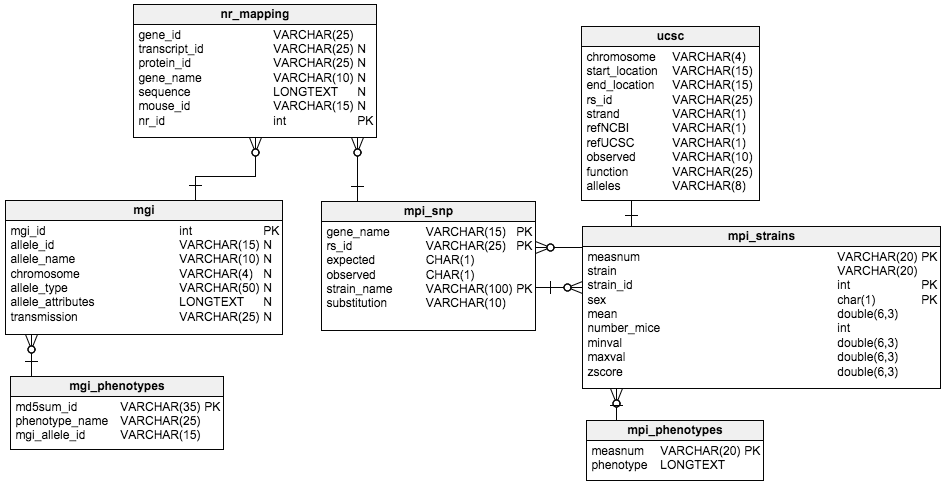
\includegraphics[width=\linewidth]{pics/db.png}
	\captionsetup{margin=12pt,format=plain,font=footnotesize,labelfont=bf}
 	\caption{\footnotesize{\textbf{MGI phenotypes}. 
	~~~~~~~\\
	The database created with information of MGI, MPI and UCSC.}}
	\label{fig:database}
\end{figure}

%------------------------------------------------

\section{Results}

\begin{figure}[H]
	\centering
	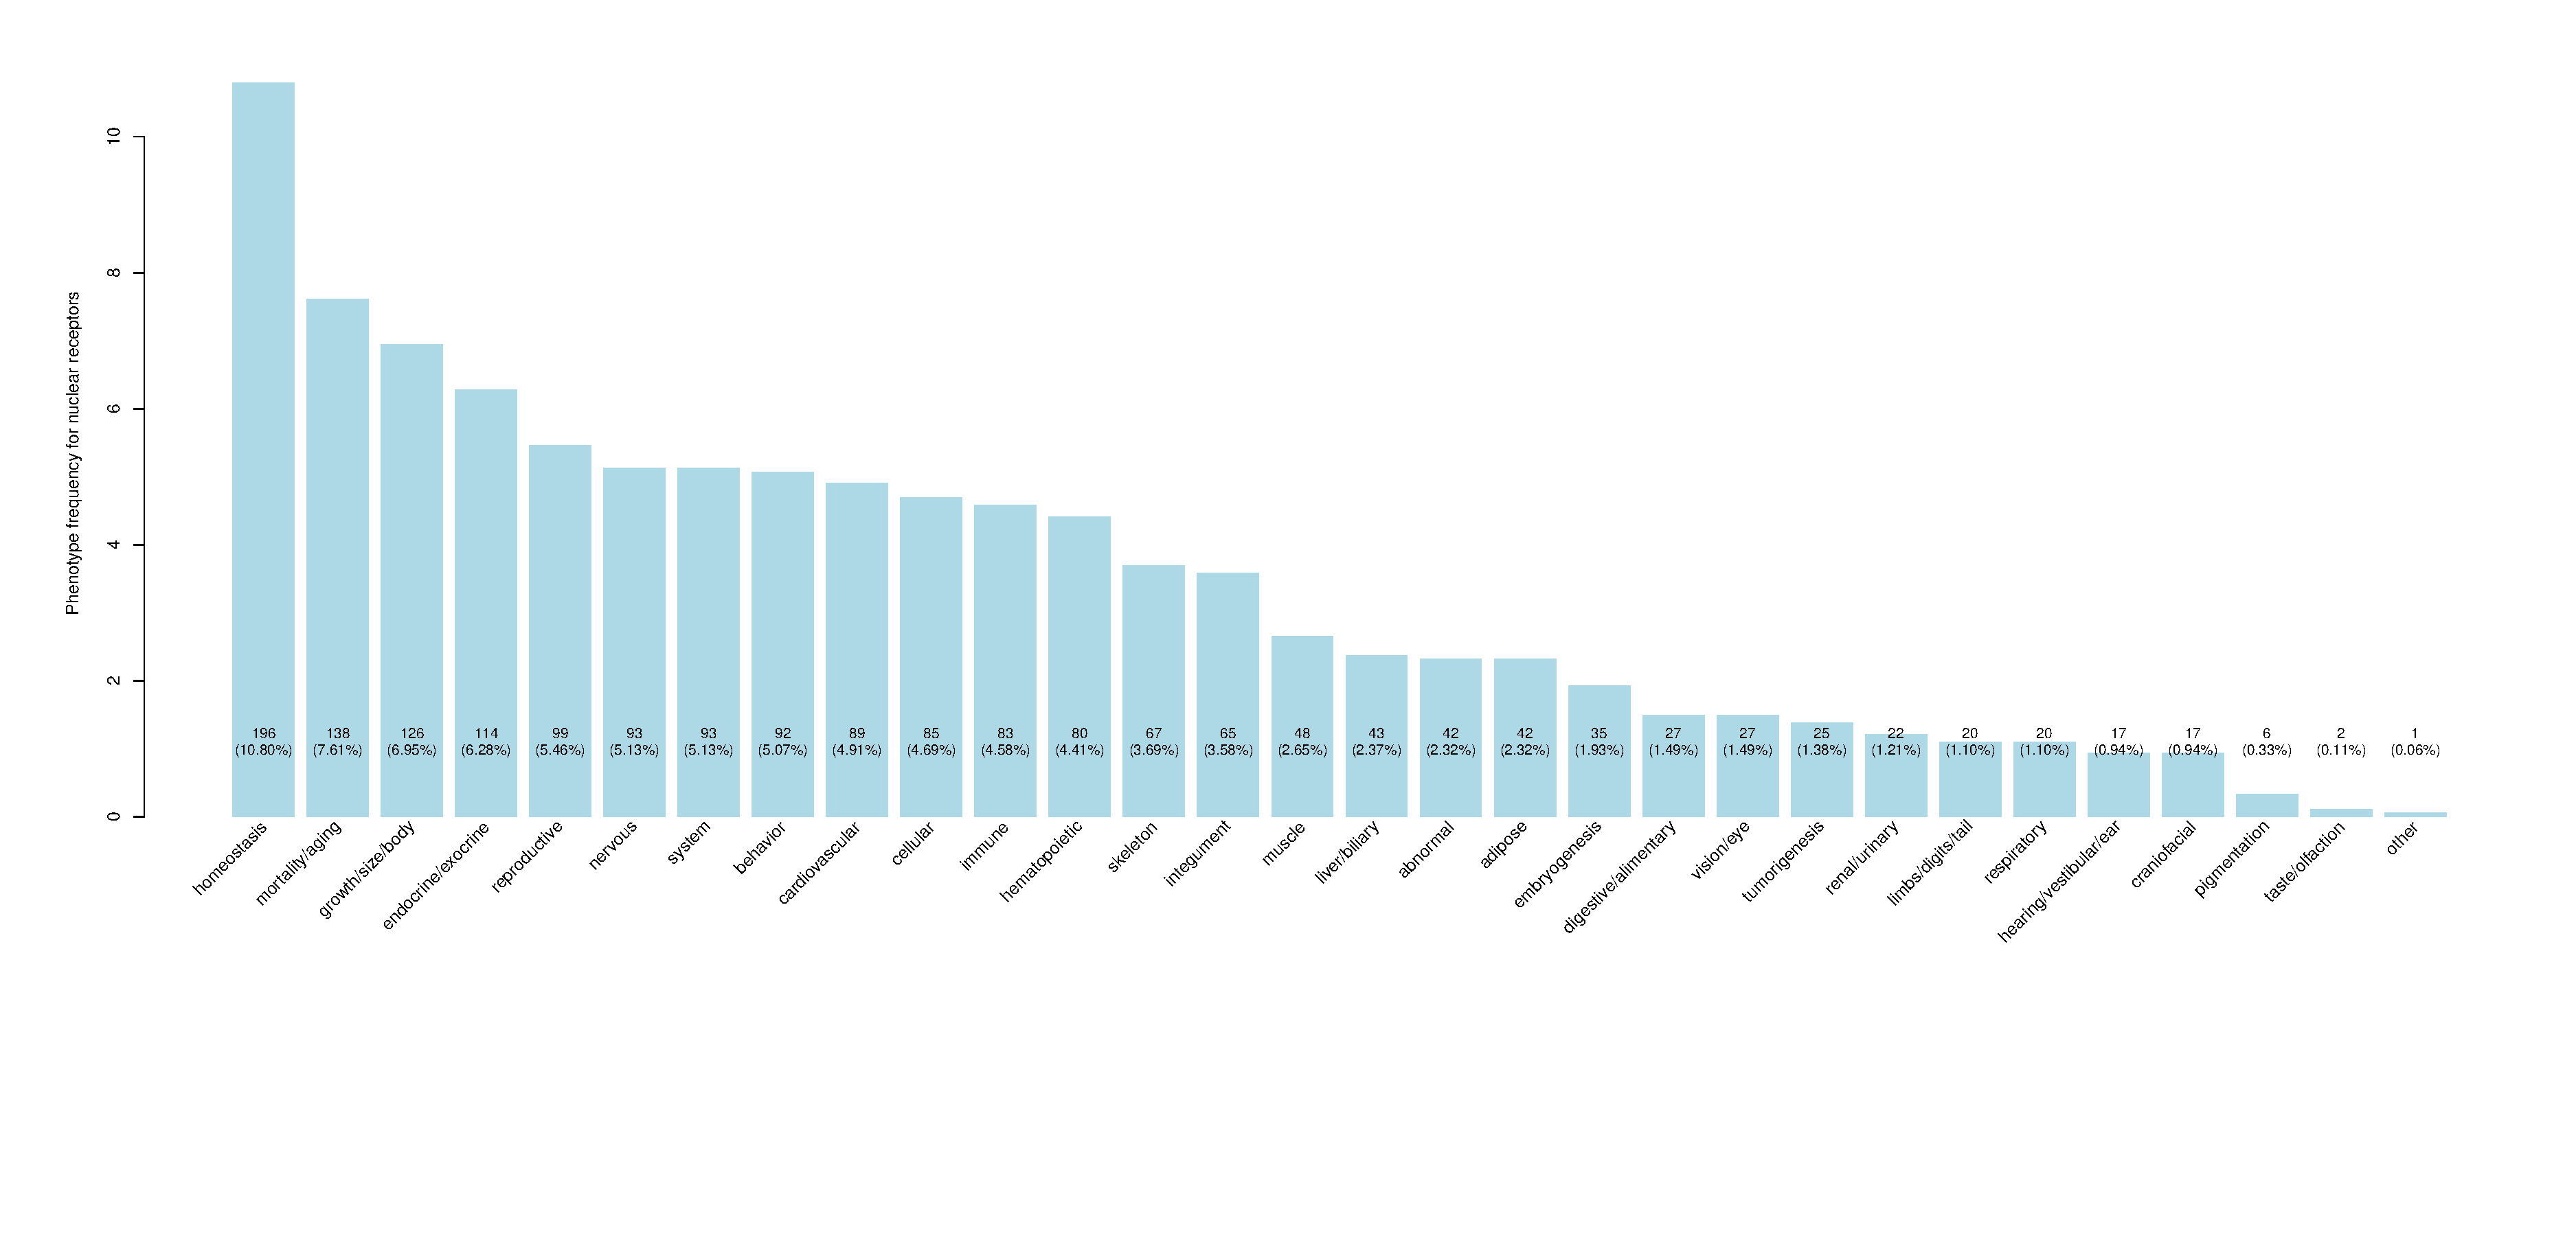
\includegraphics[width=\linewidth]{pics/mgi_phenotypes_distribution.pdf}
	\captionsetup{margin=12pt,format=plain,font=footnotesize,labelfont=bf}
 	\caption{\footnotesize{\textbf{MGI phenotypes}. 
	~~~~~~~\\
	Mouse Genome Informatics phenotype distribution over the nuclear receptors.}}
	\label{fig:mgi_pheotypes_distribution}
\end{figure}
~~~~~~~\\

%Figure~\ref{fig:mgi_pheotypes_distribution} bla bla 
\begin{figure}[H]
	\centering
	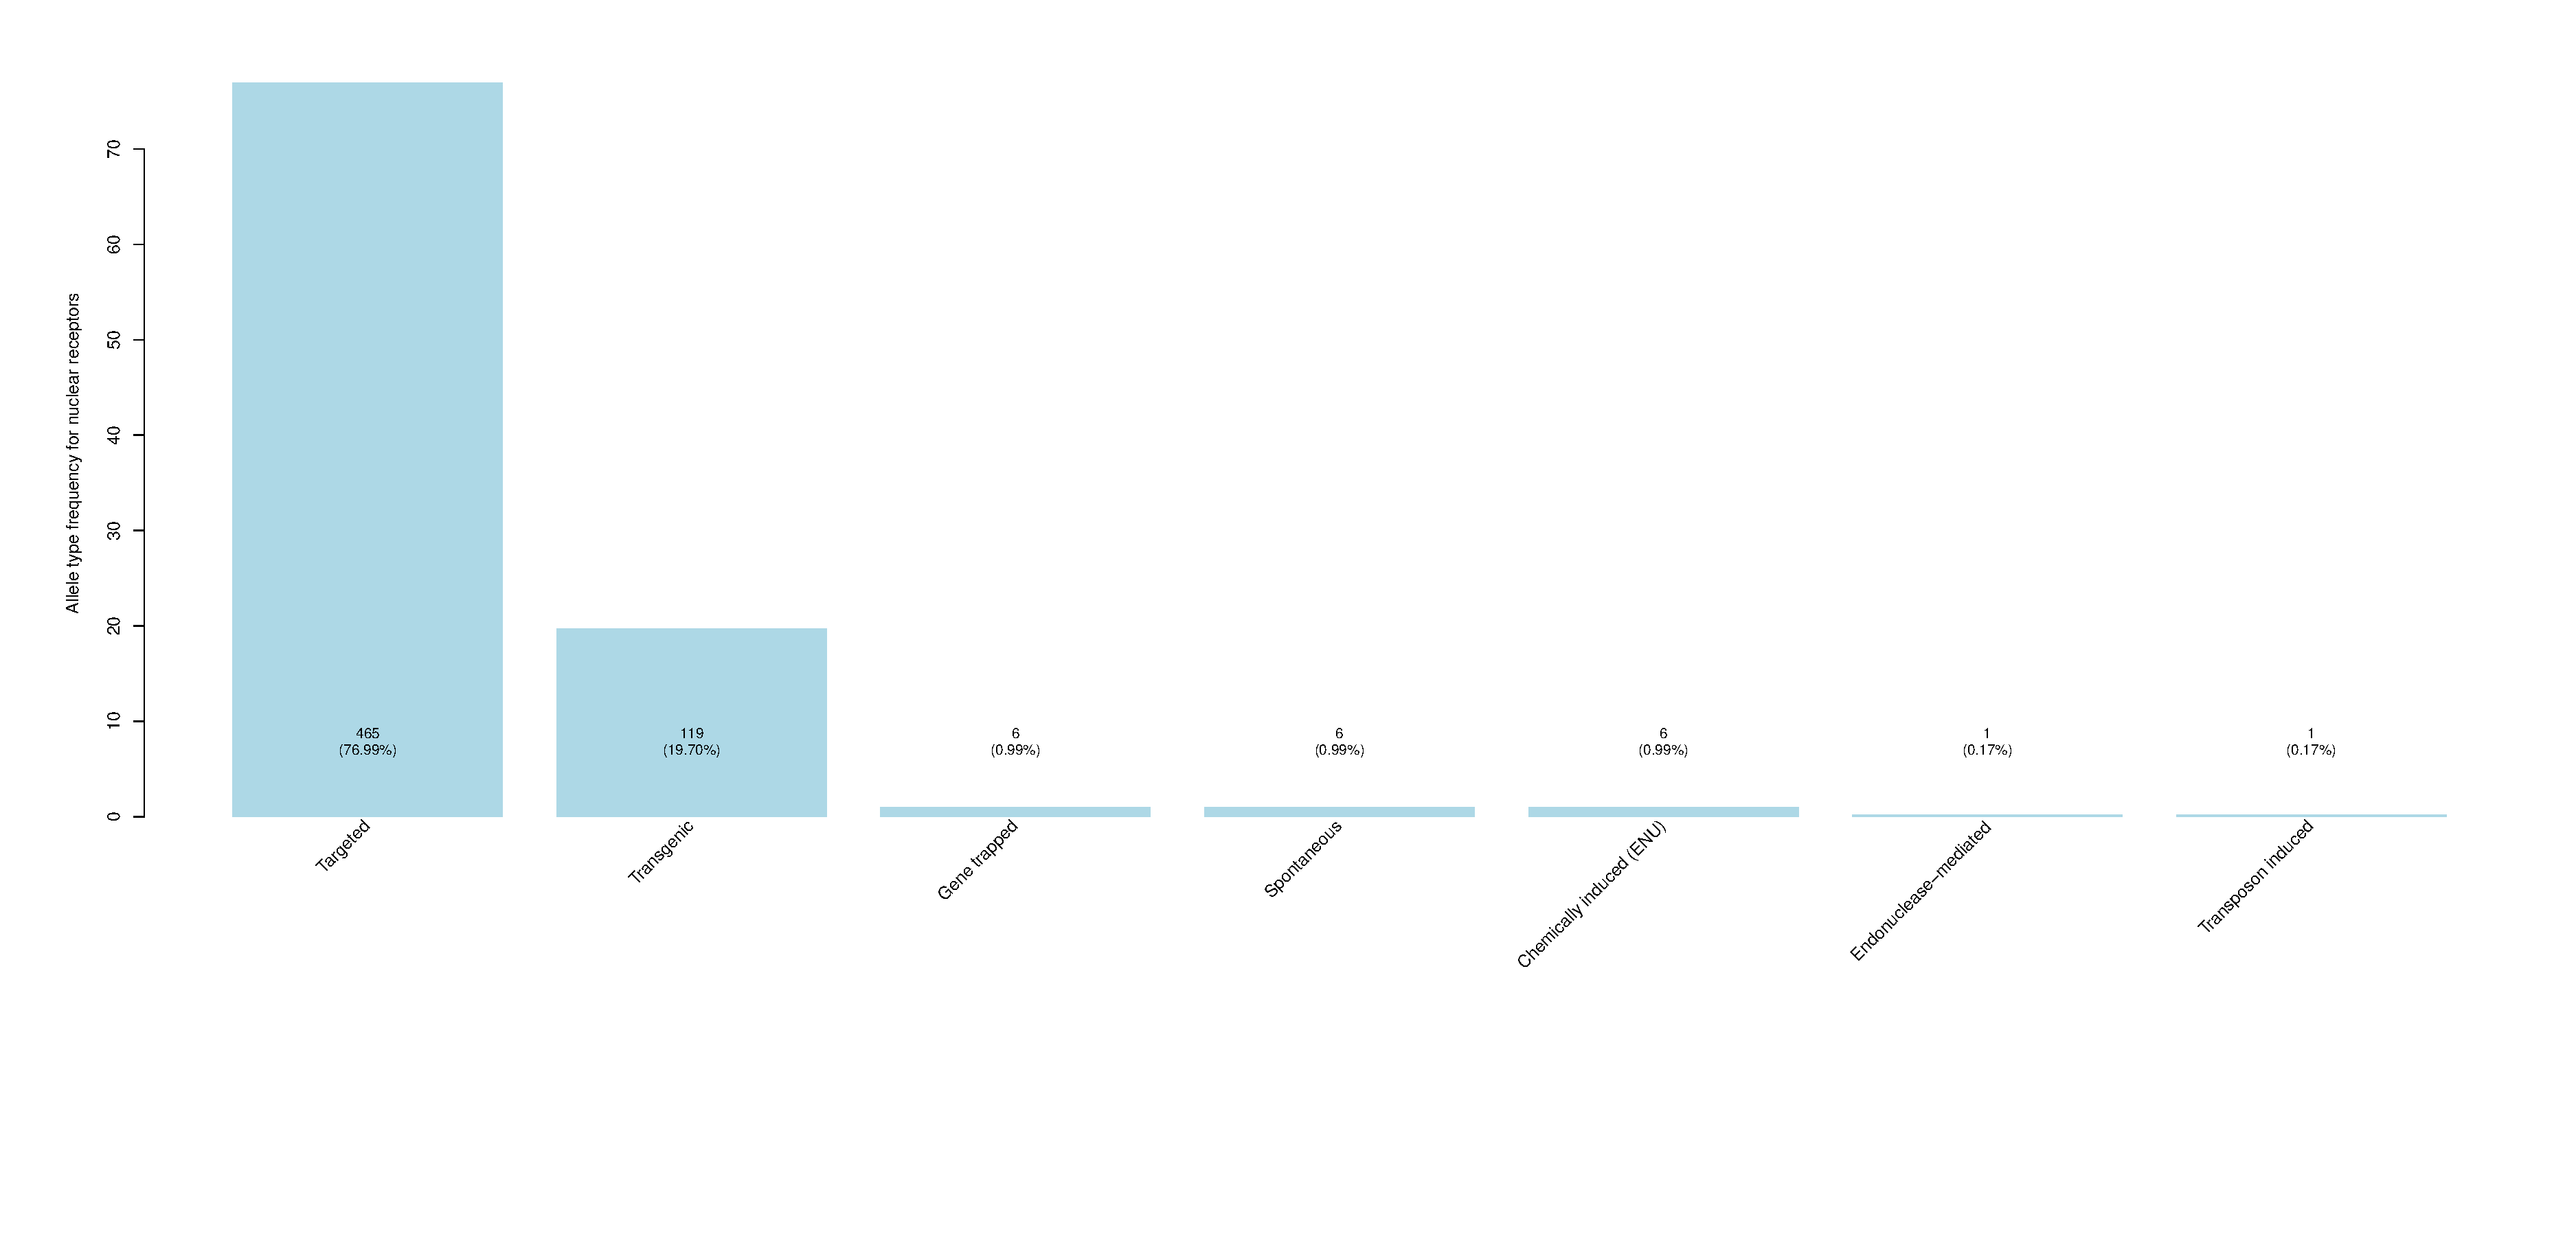
\includegraphics[width=\linewidth]{pics/mgi_types_distribution.pdf}
	\captionsetup{margin=12pt,format=plain,font=footnotesize,labelfont=bf}
 	\caption{\footnotesize{\textbf{MGI allele types}. 
	~~~~~~~\\
	Mouse Genome Informatics allele type distribution over the nuclear receptors.}}
	\label{fig:mgi_types_distribution}
\end{figure}
~~~~~~~\\

\begin{figure}[H]
	\centering
	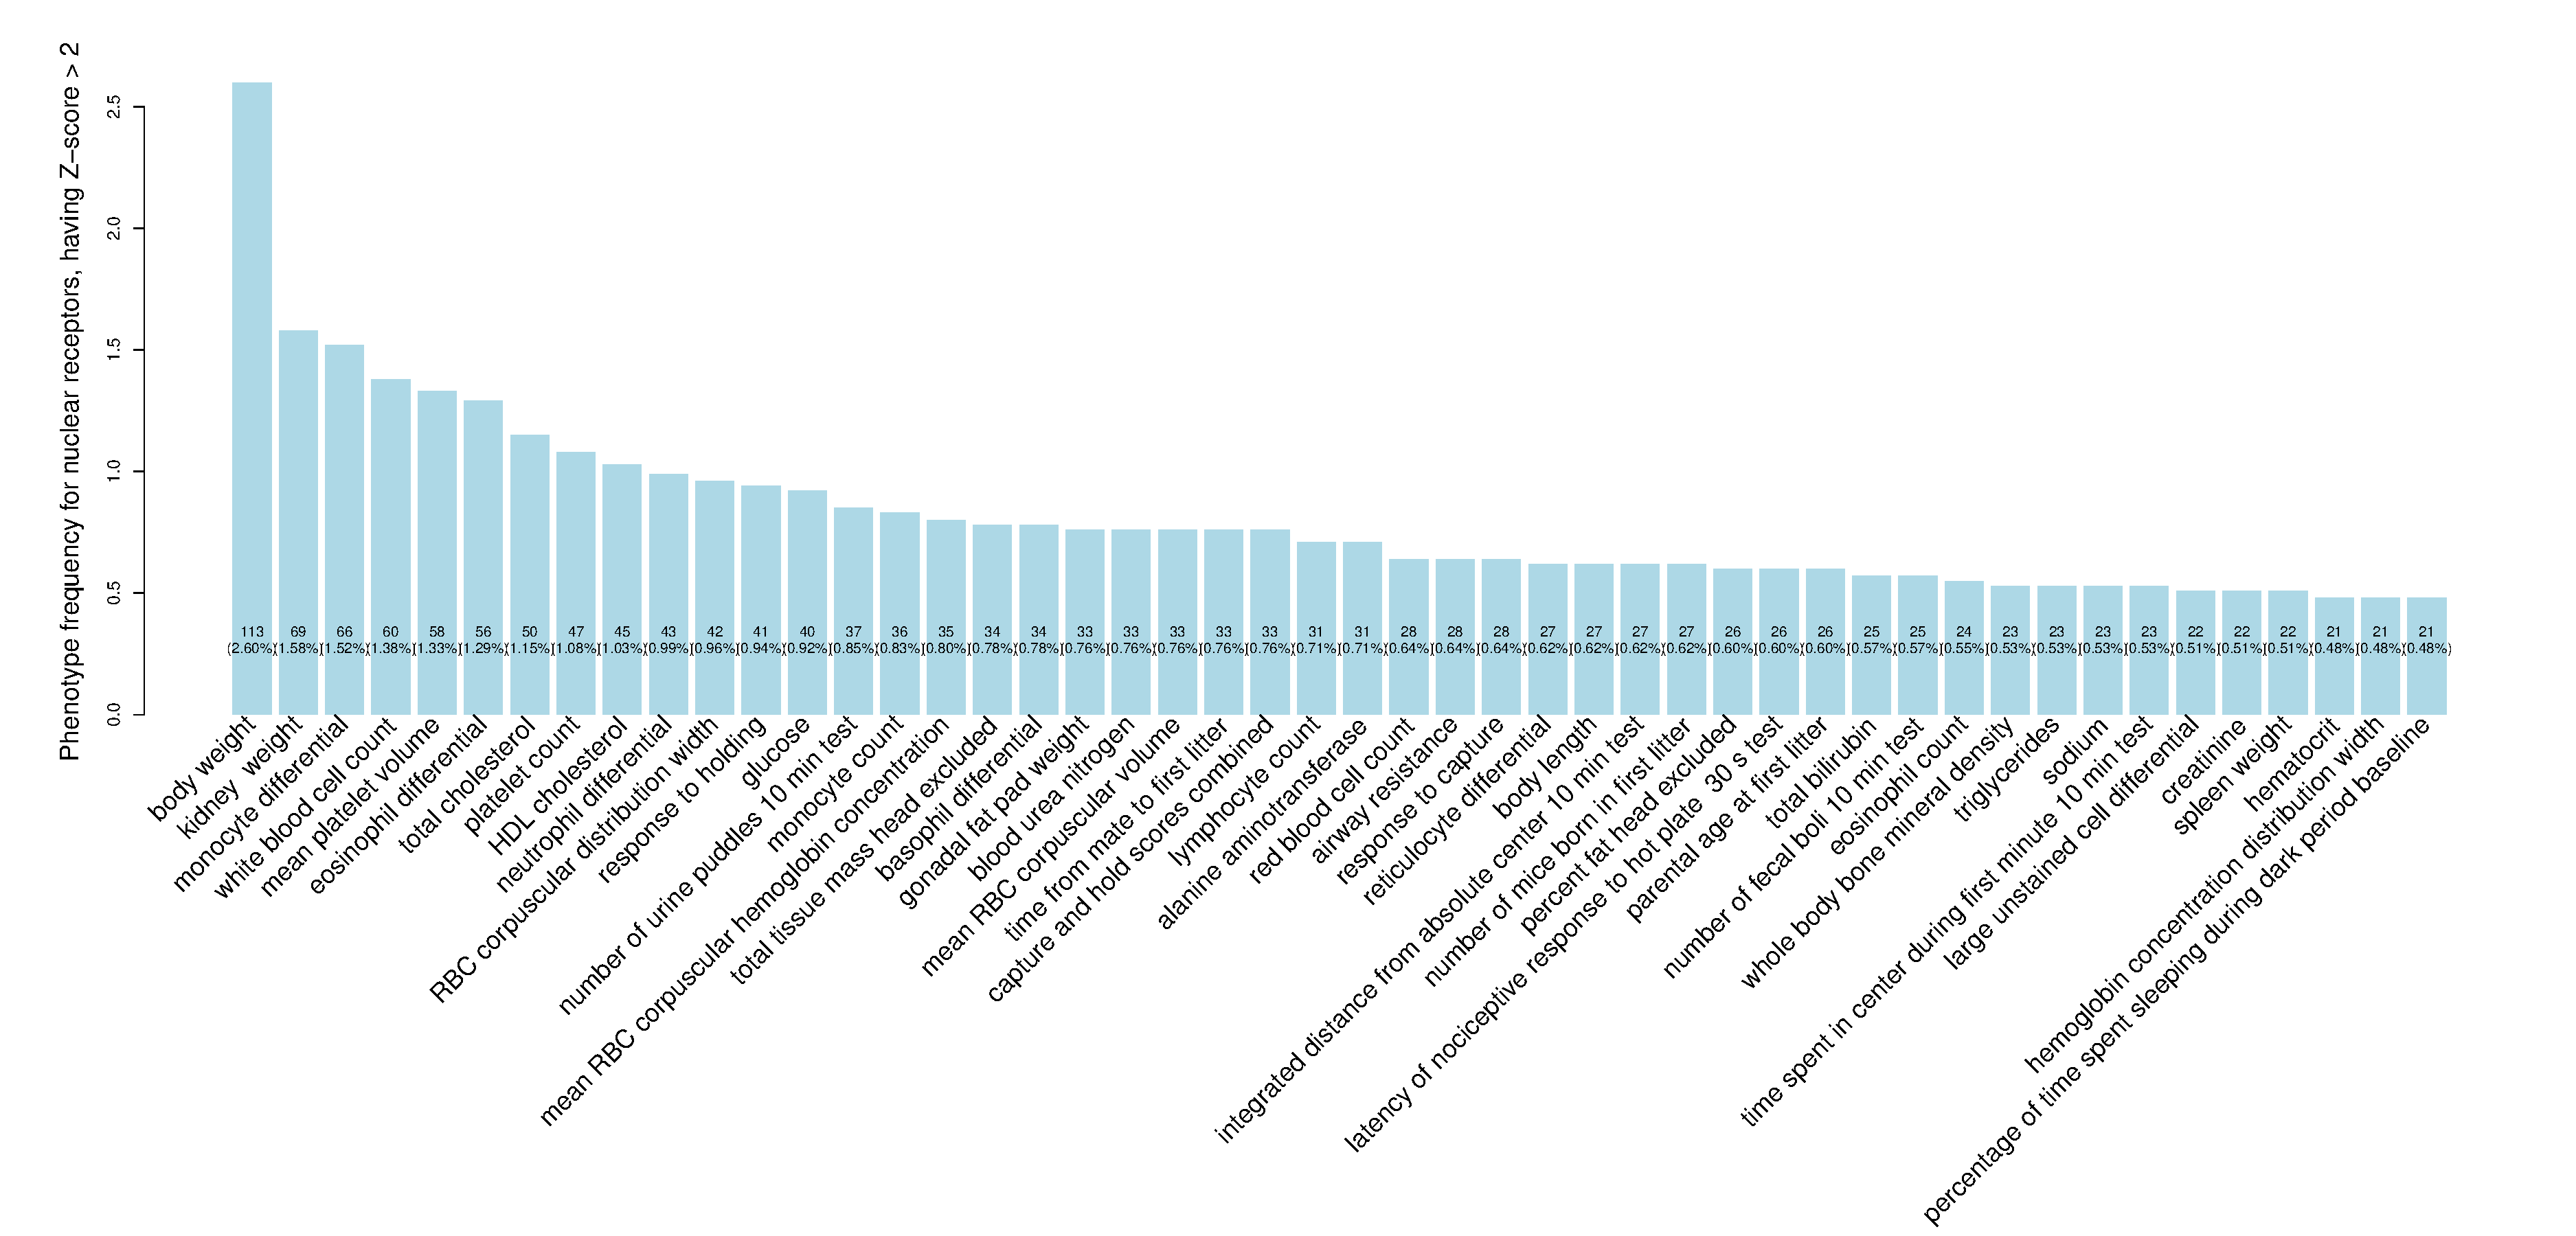
\includegraphics[width=\linewidth]{pics/mpi_phenotypes_distribution_zscore2.pdf}
	\captionsetup{margin=12pt,format=plain,font=footnotesize,labelfont=bf}
 	\caption{\footnotesize{\textbf{MPD phenotypes, having Z-score $>$ 2}. 
	~~~~~~~\\
	Mouse Phenotype Database phenotype distribution over the nuclear receptors, having Z-score $>$ 2}}
	\label{fig:mpi_pheotypes_distribution_zscore2}
\end{figure}
~~~~~~~\\

\begin{figure}[H]
	\centering
	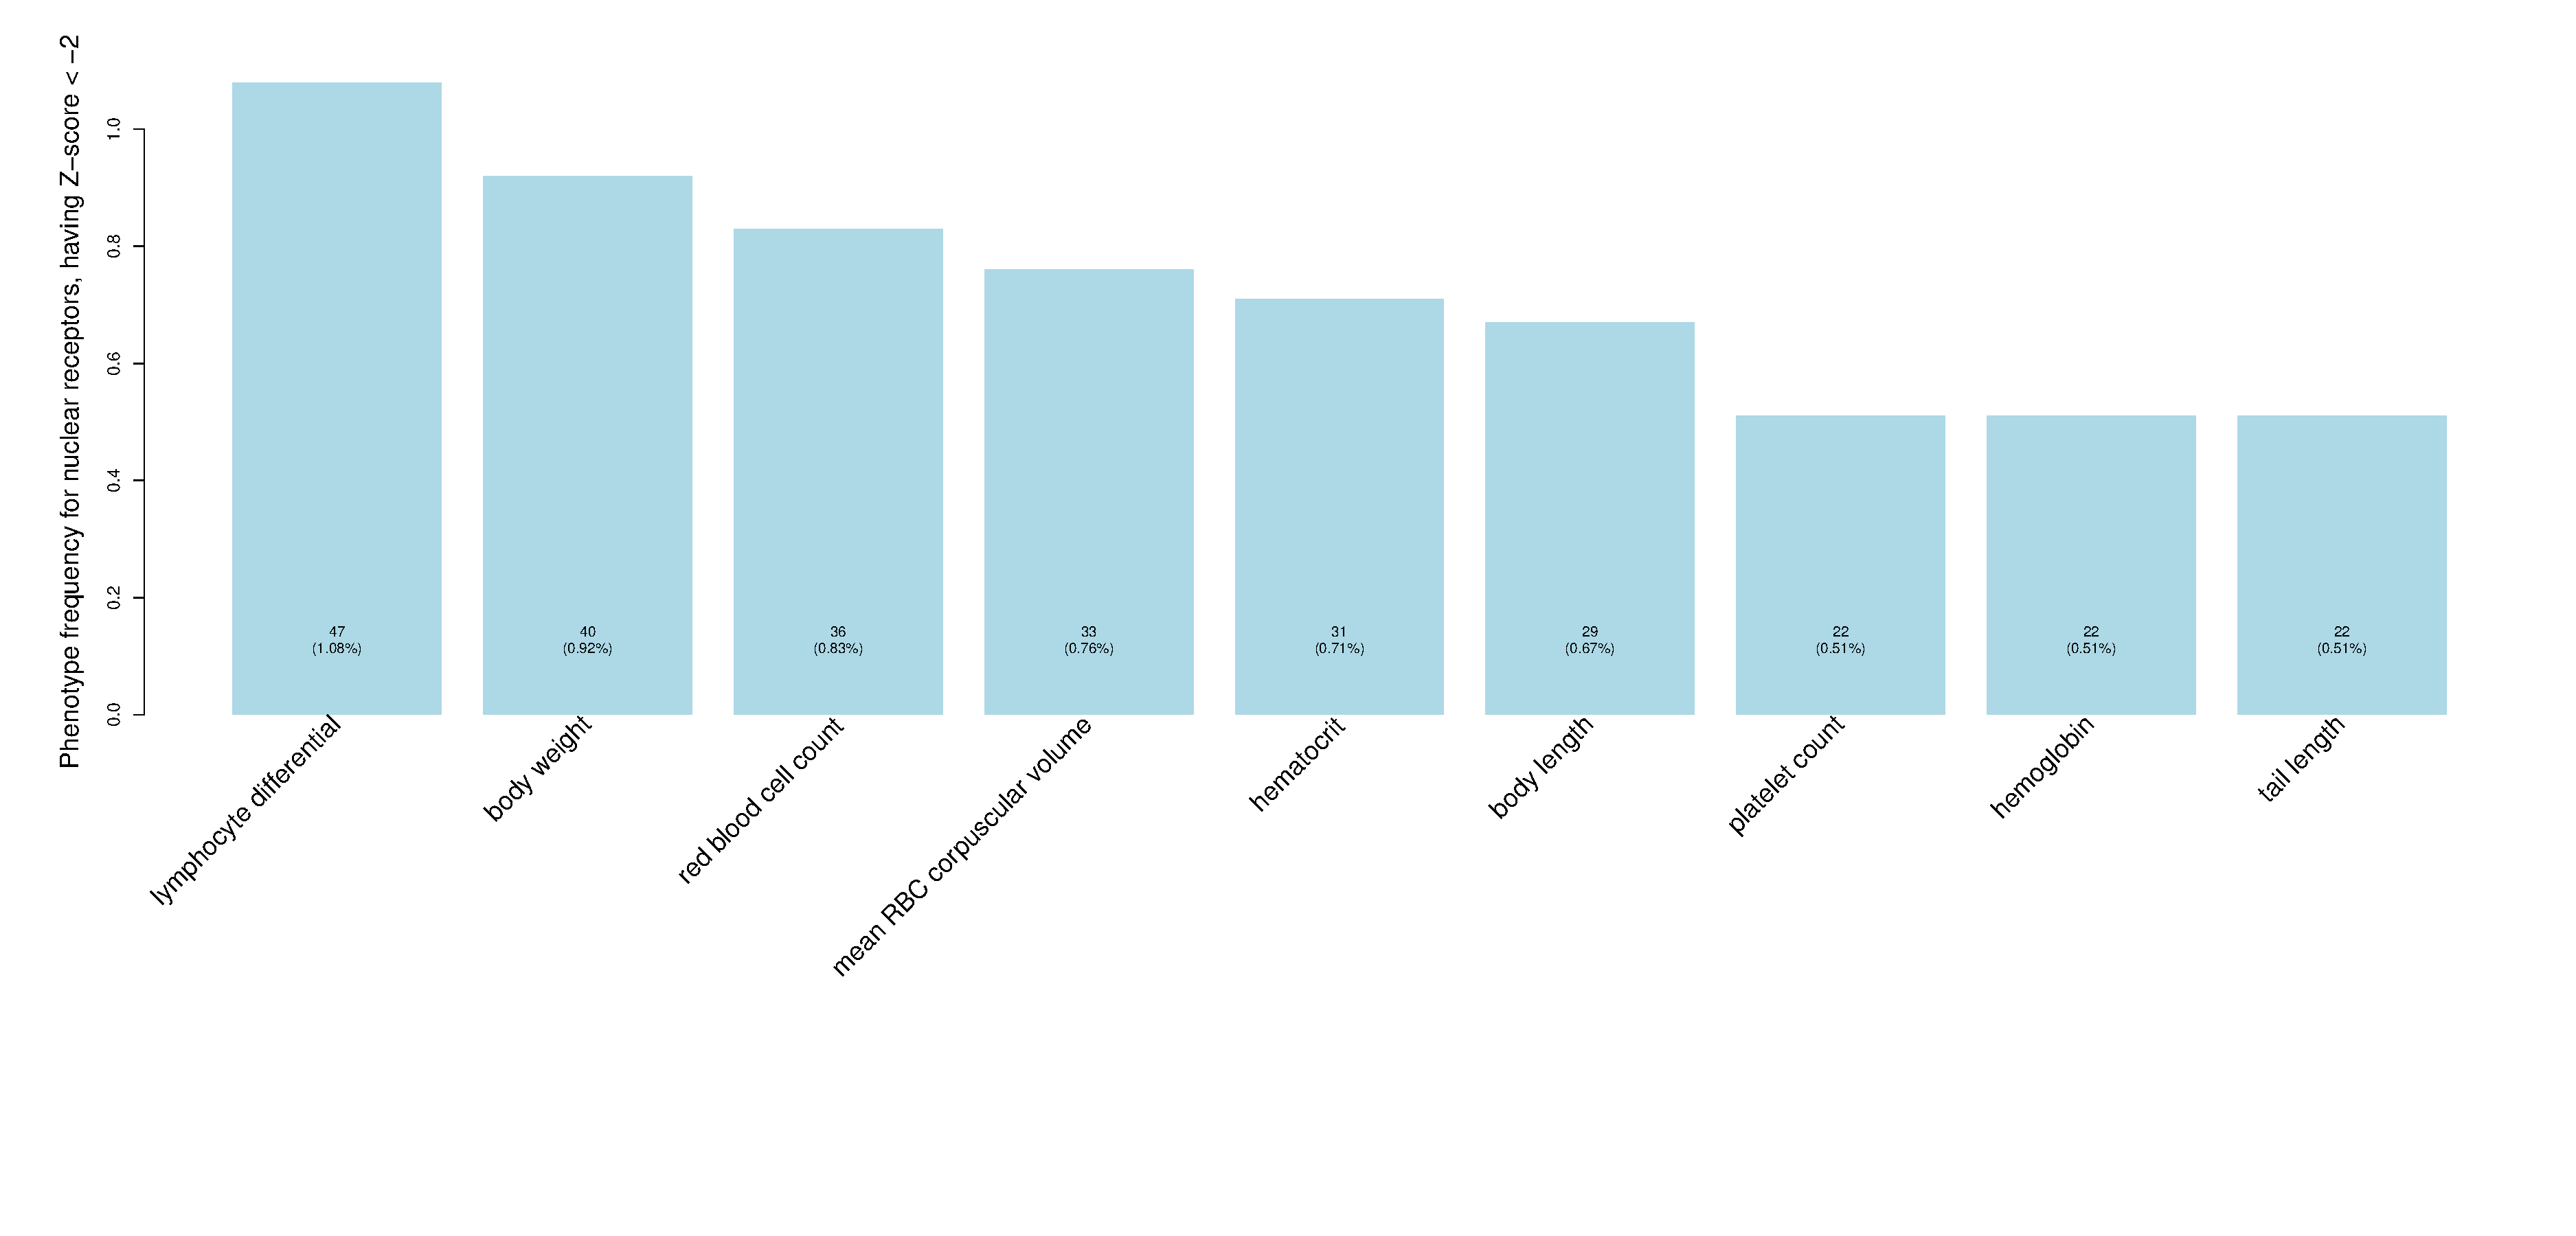
\includegraphics[width=\linewidth]{pics/mpi_phenotypes_distribution_zscore2_neg.pdf}
	\captionsetup{margin=12pt,format=plain,font=footnotesize,labelfont=bf}
 	\caption{\footnotesize{\textbf{MPD phenotypes, having Z-score $<$ -2}. 
	~~~~~~~\\
	Mouse Phenotype Database phenotype distribution over the nuclear receptors, having Z-score $<$ -2}}
	\label{fig:mpi_pheotypes_distribution_zscore2_neg}
\end{figure}
~~~~~~~\\

\begin{figure}[H]
	\centering
	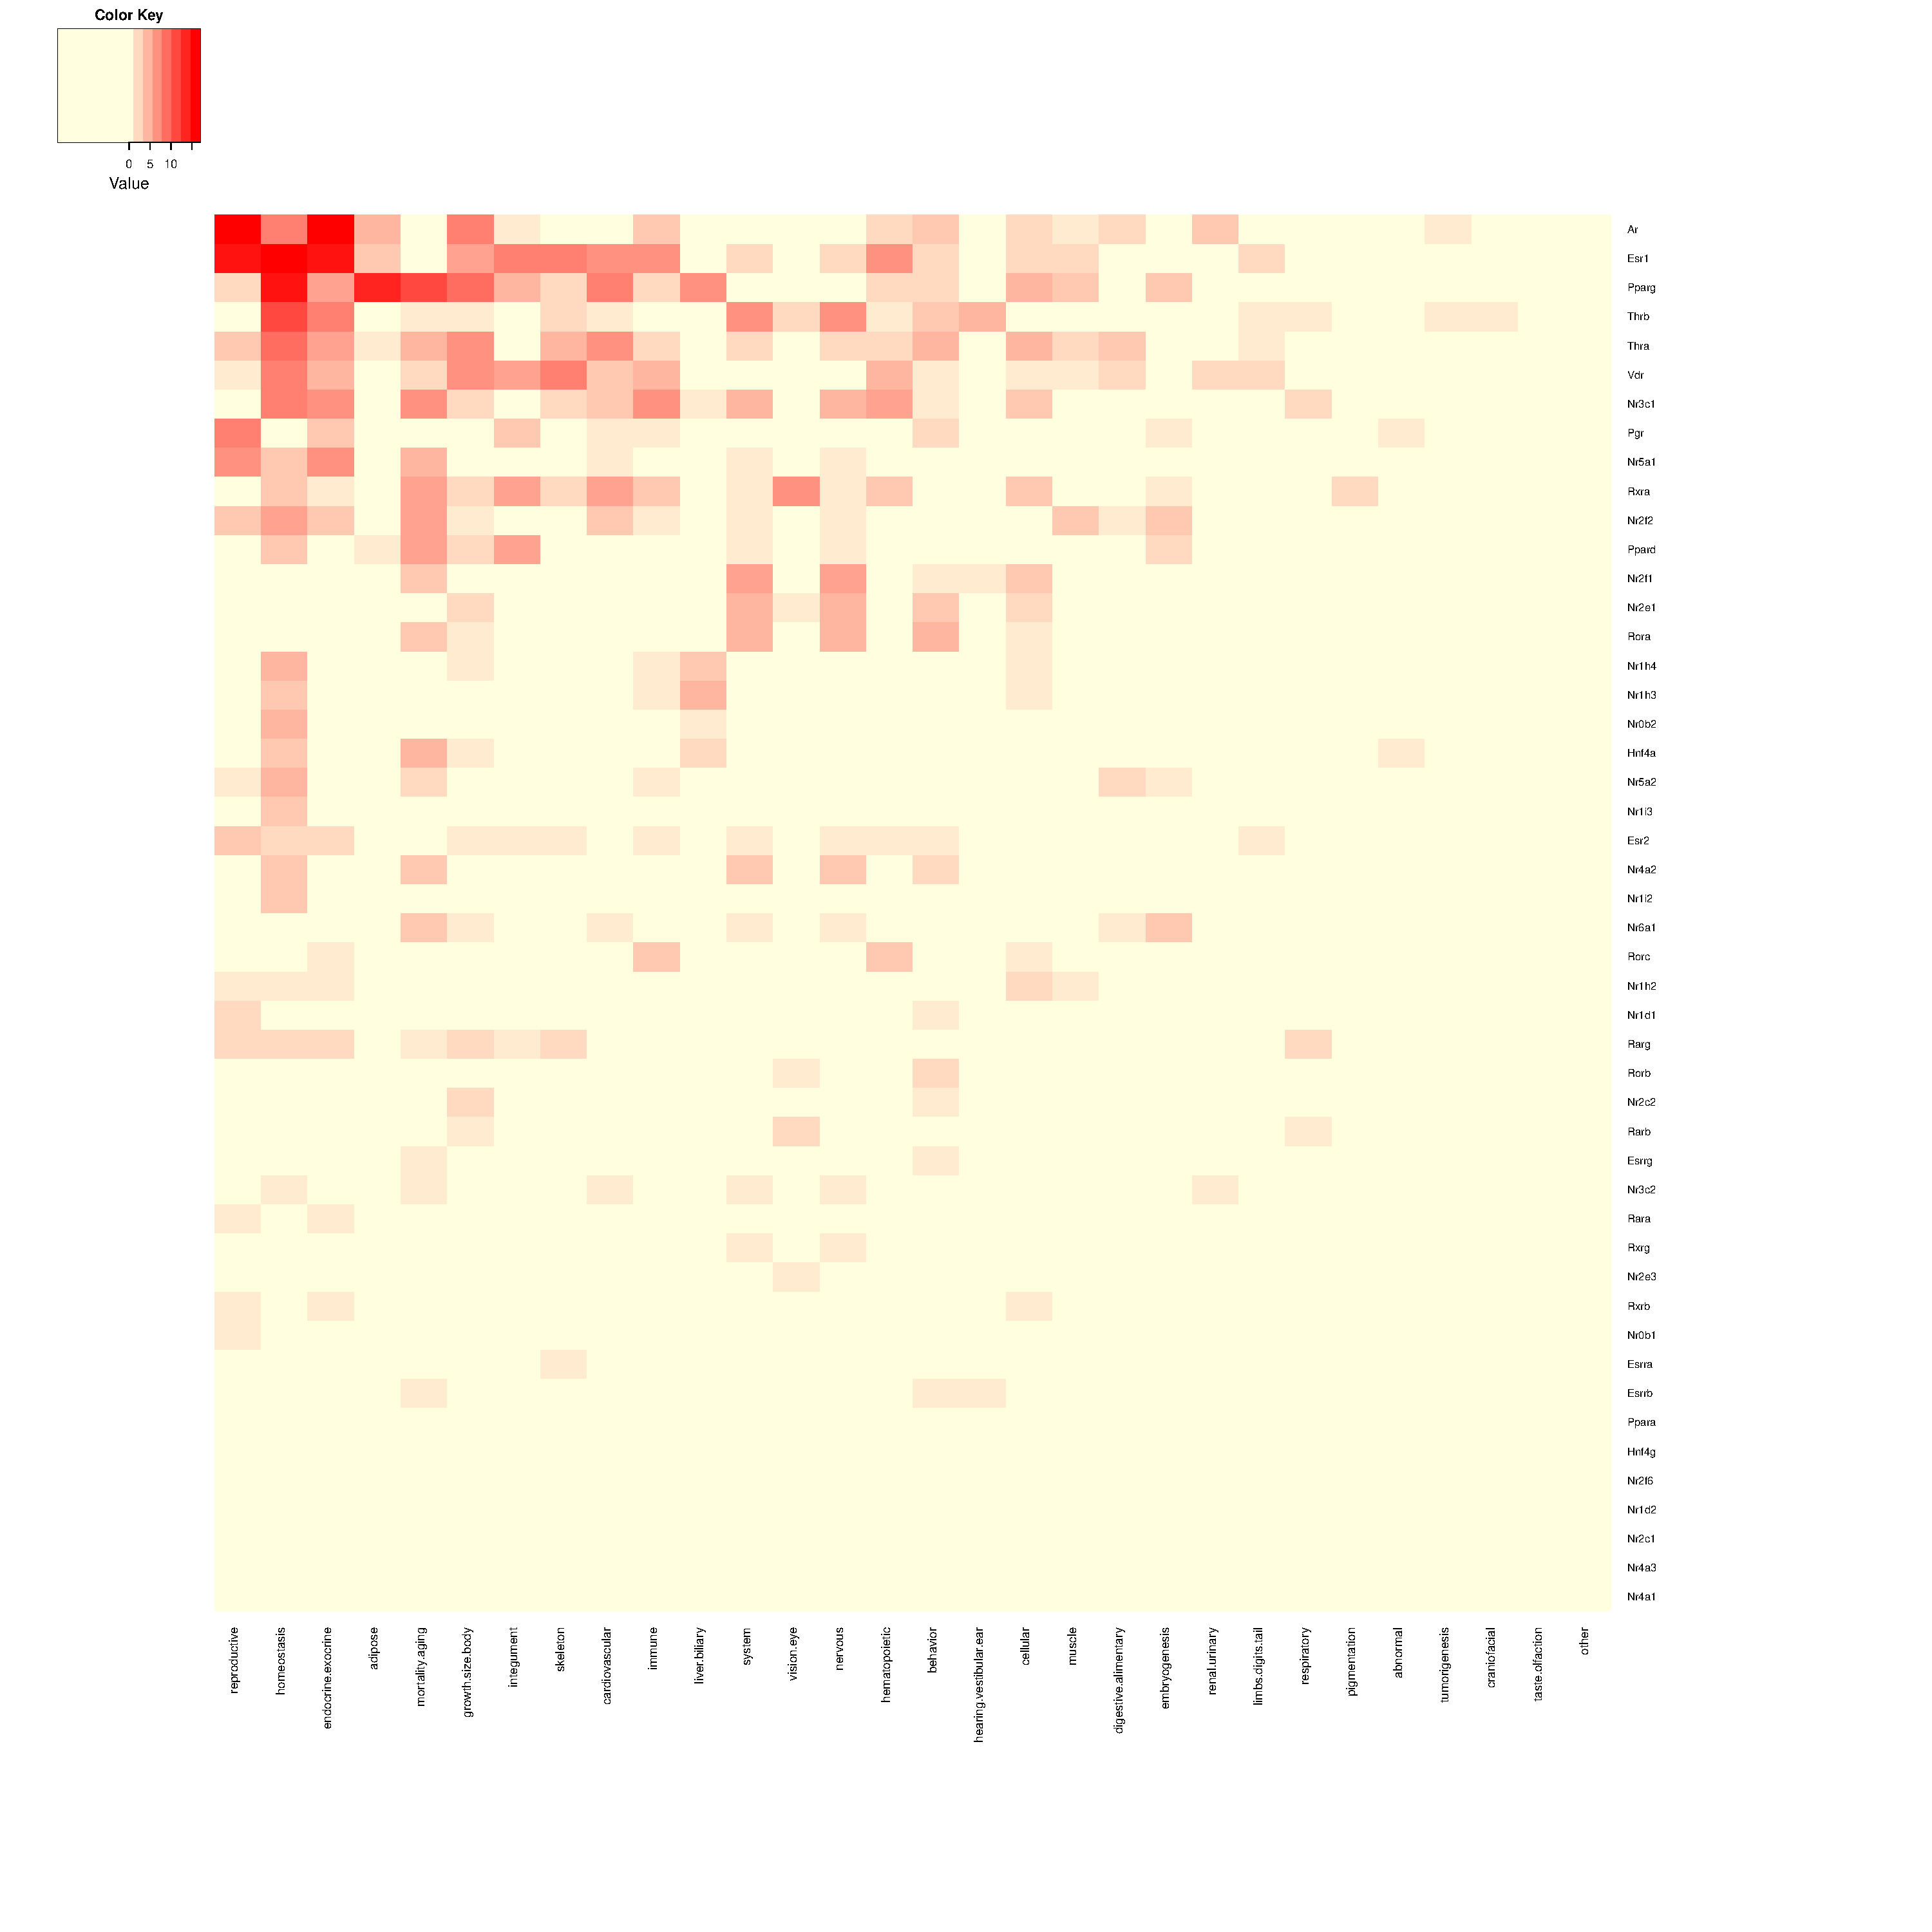
\includegraphics[width=\linewidth]{pics/mgi_phenotypes_nr.pdf}
	\captionsetup{margin=12pt,format=plain,font=footnotesize,labelfont=bf}
 	\caption{\footnotesize{\textbf{MGI phenotype - nuclear receptor associations}. 
	~~~~~~~\\
	Mouse Genome Informatics phenotype occurrence frequency among the nuclear receptors.}}
	\label{fig:mgi_pheotypes_nr}
\end{figure}
~~~~~~~\\

\begin{figure}[H]
	\centering
	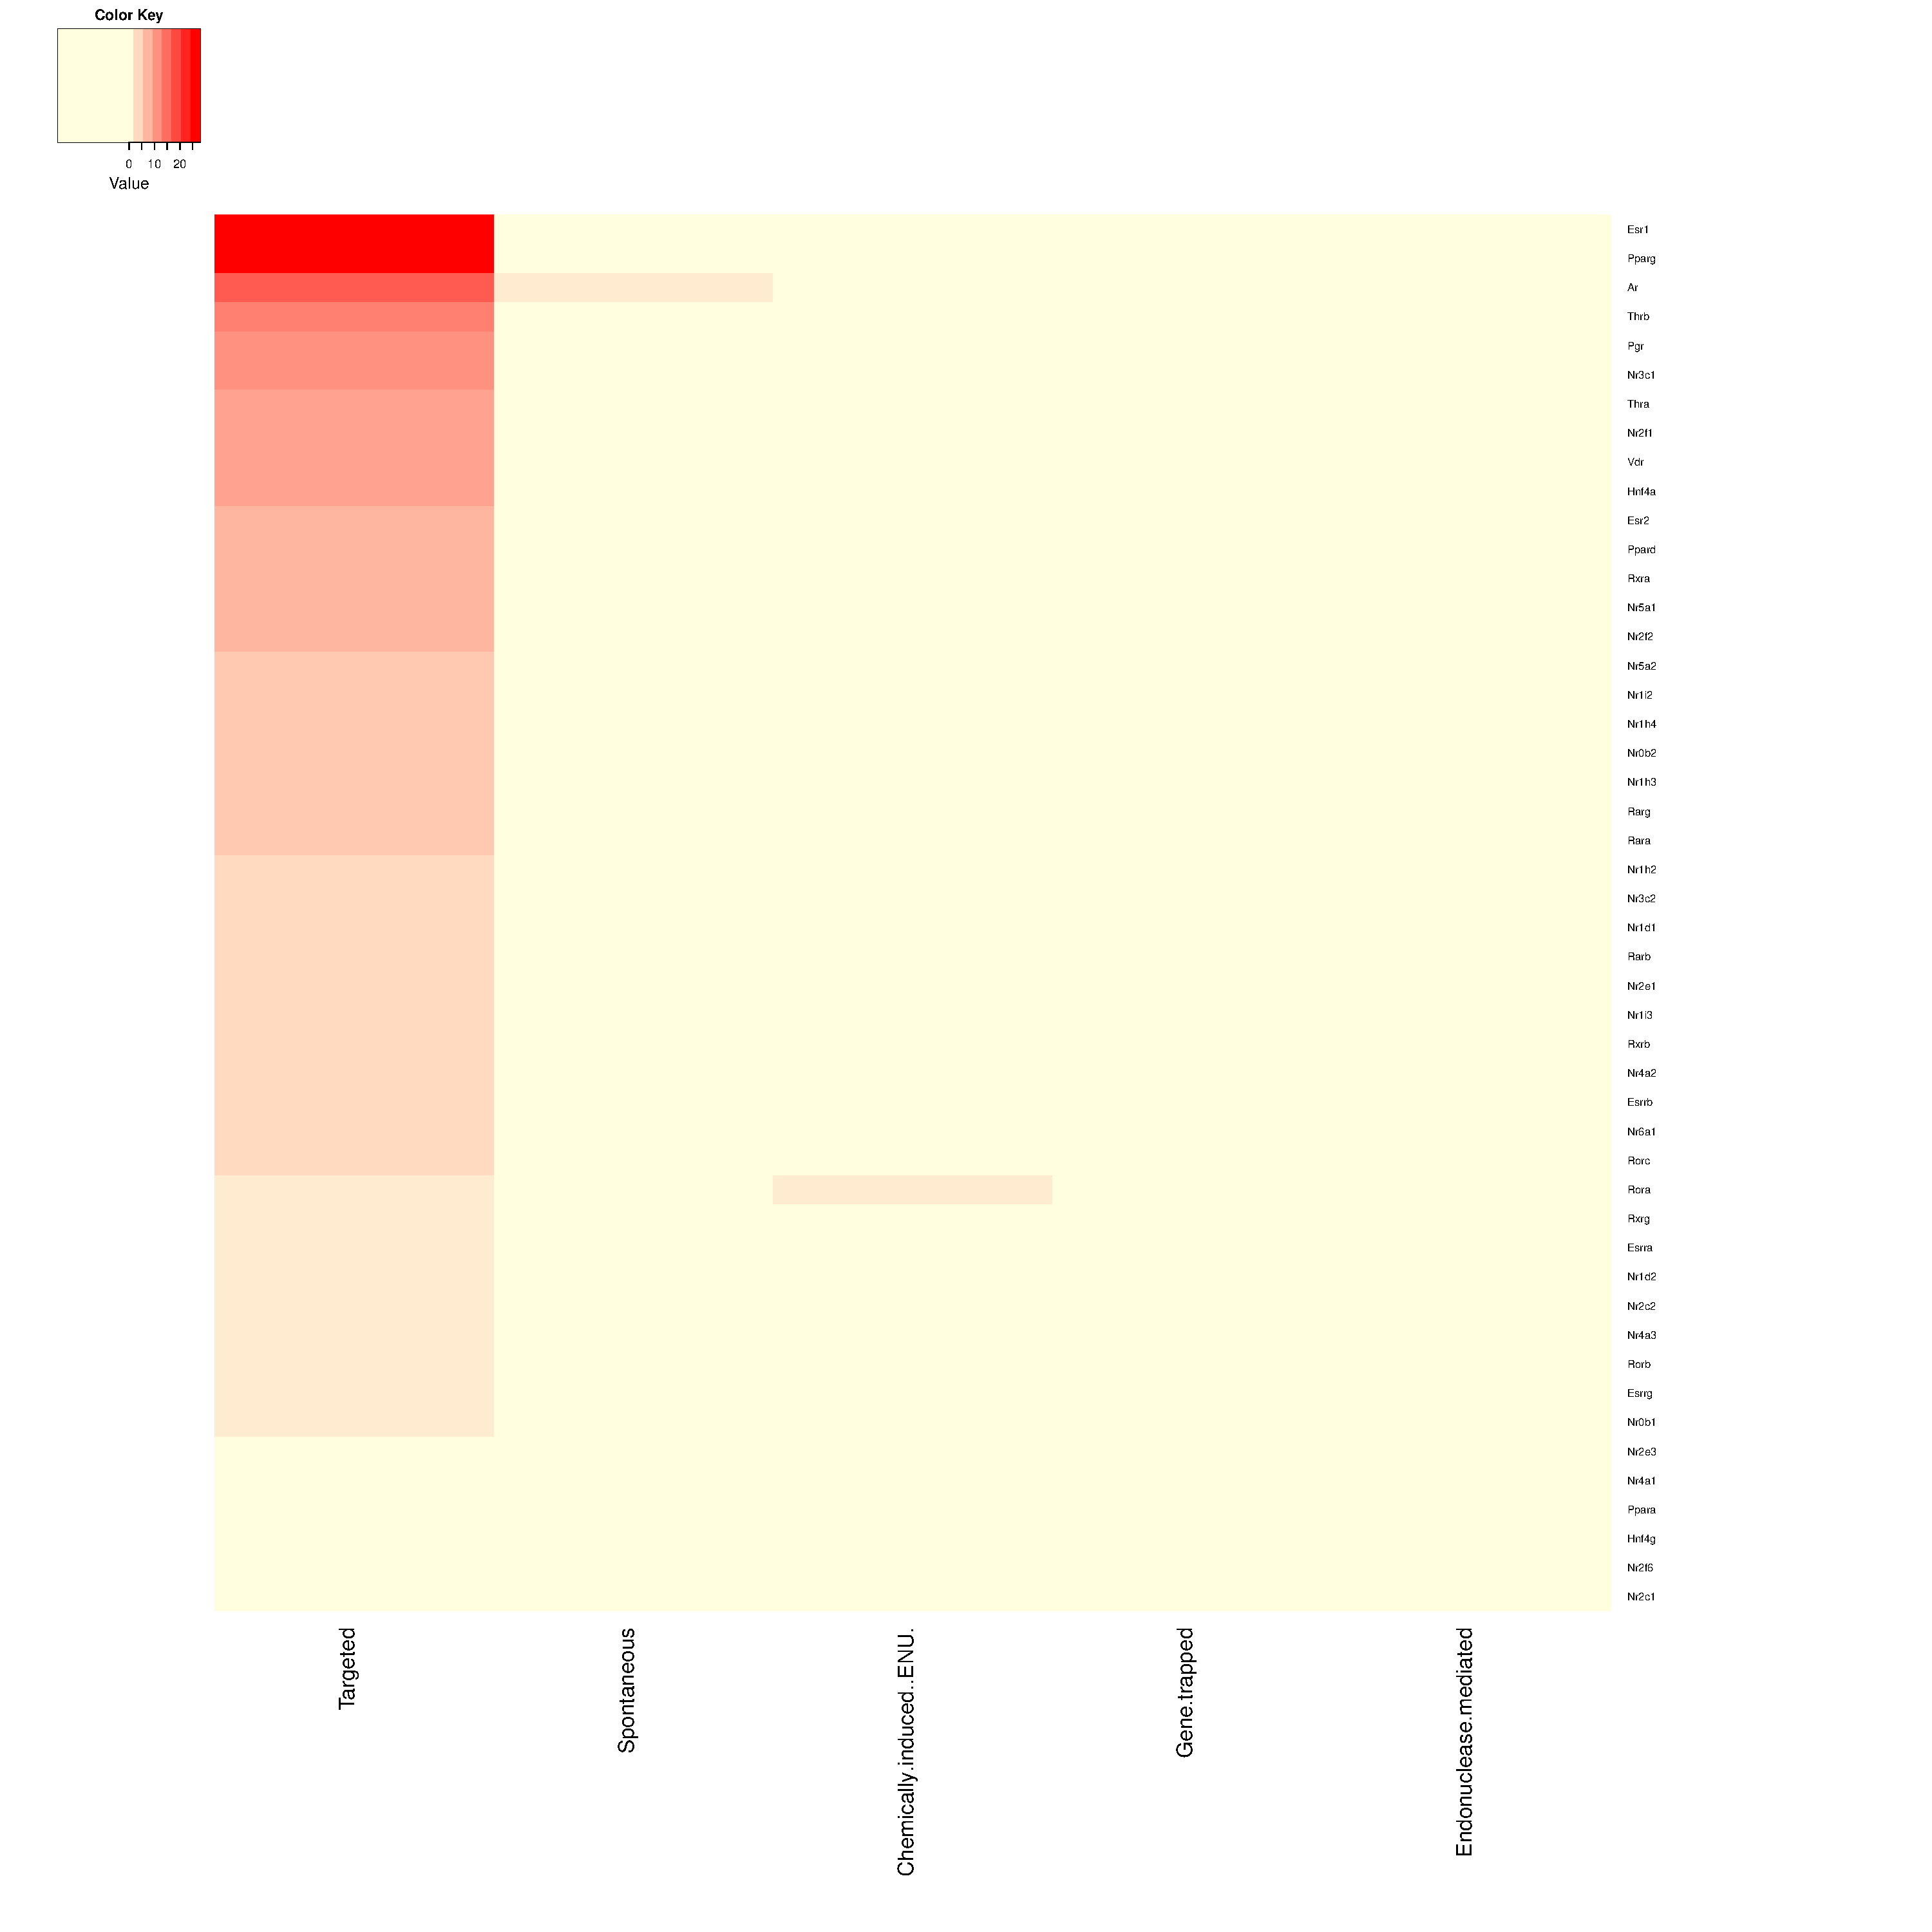
\includegraphics[width=\linewidth]{pics/mgi_types_nr.pdf}
	\captionsetup{margin=12pt,format=plain,font=footnotesize,labelfont=bf}
 	\caption{\footnotesize{\textbf{MGI allele type - nuclear receptor associations}. 
	~~~~~~~\\
	Mouse Genome Informatics allele type occurrence frequency among the nuclear receptors.}}
	\label{fig:mgi_types_nr}
\end{figure}
~~~~~~~\\

\begin{figure}[H]
	\centering
	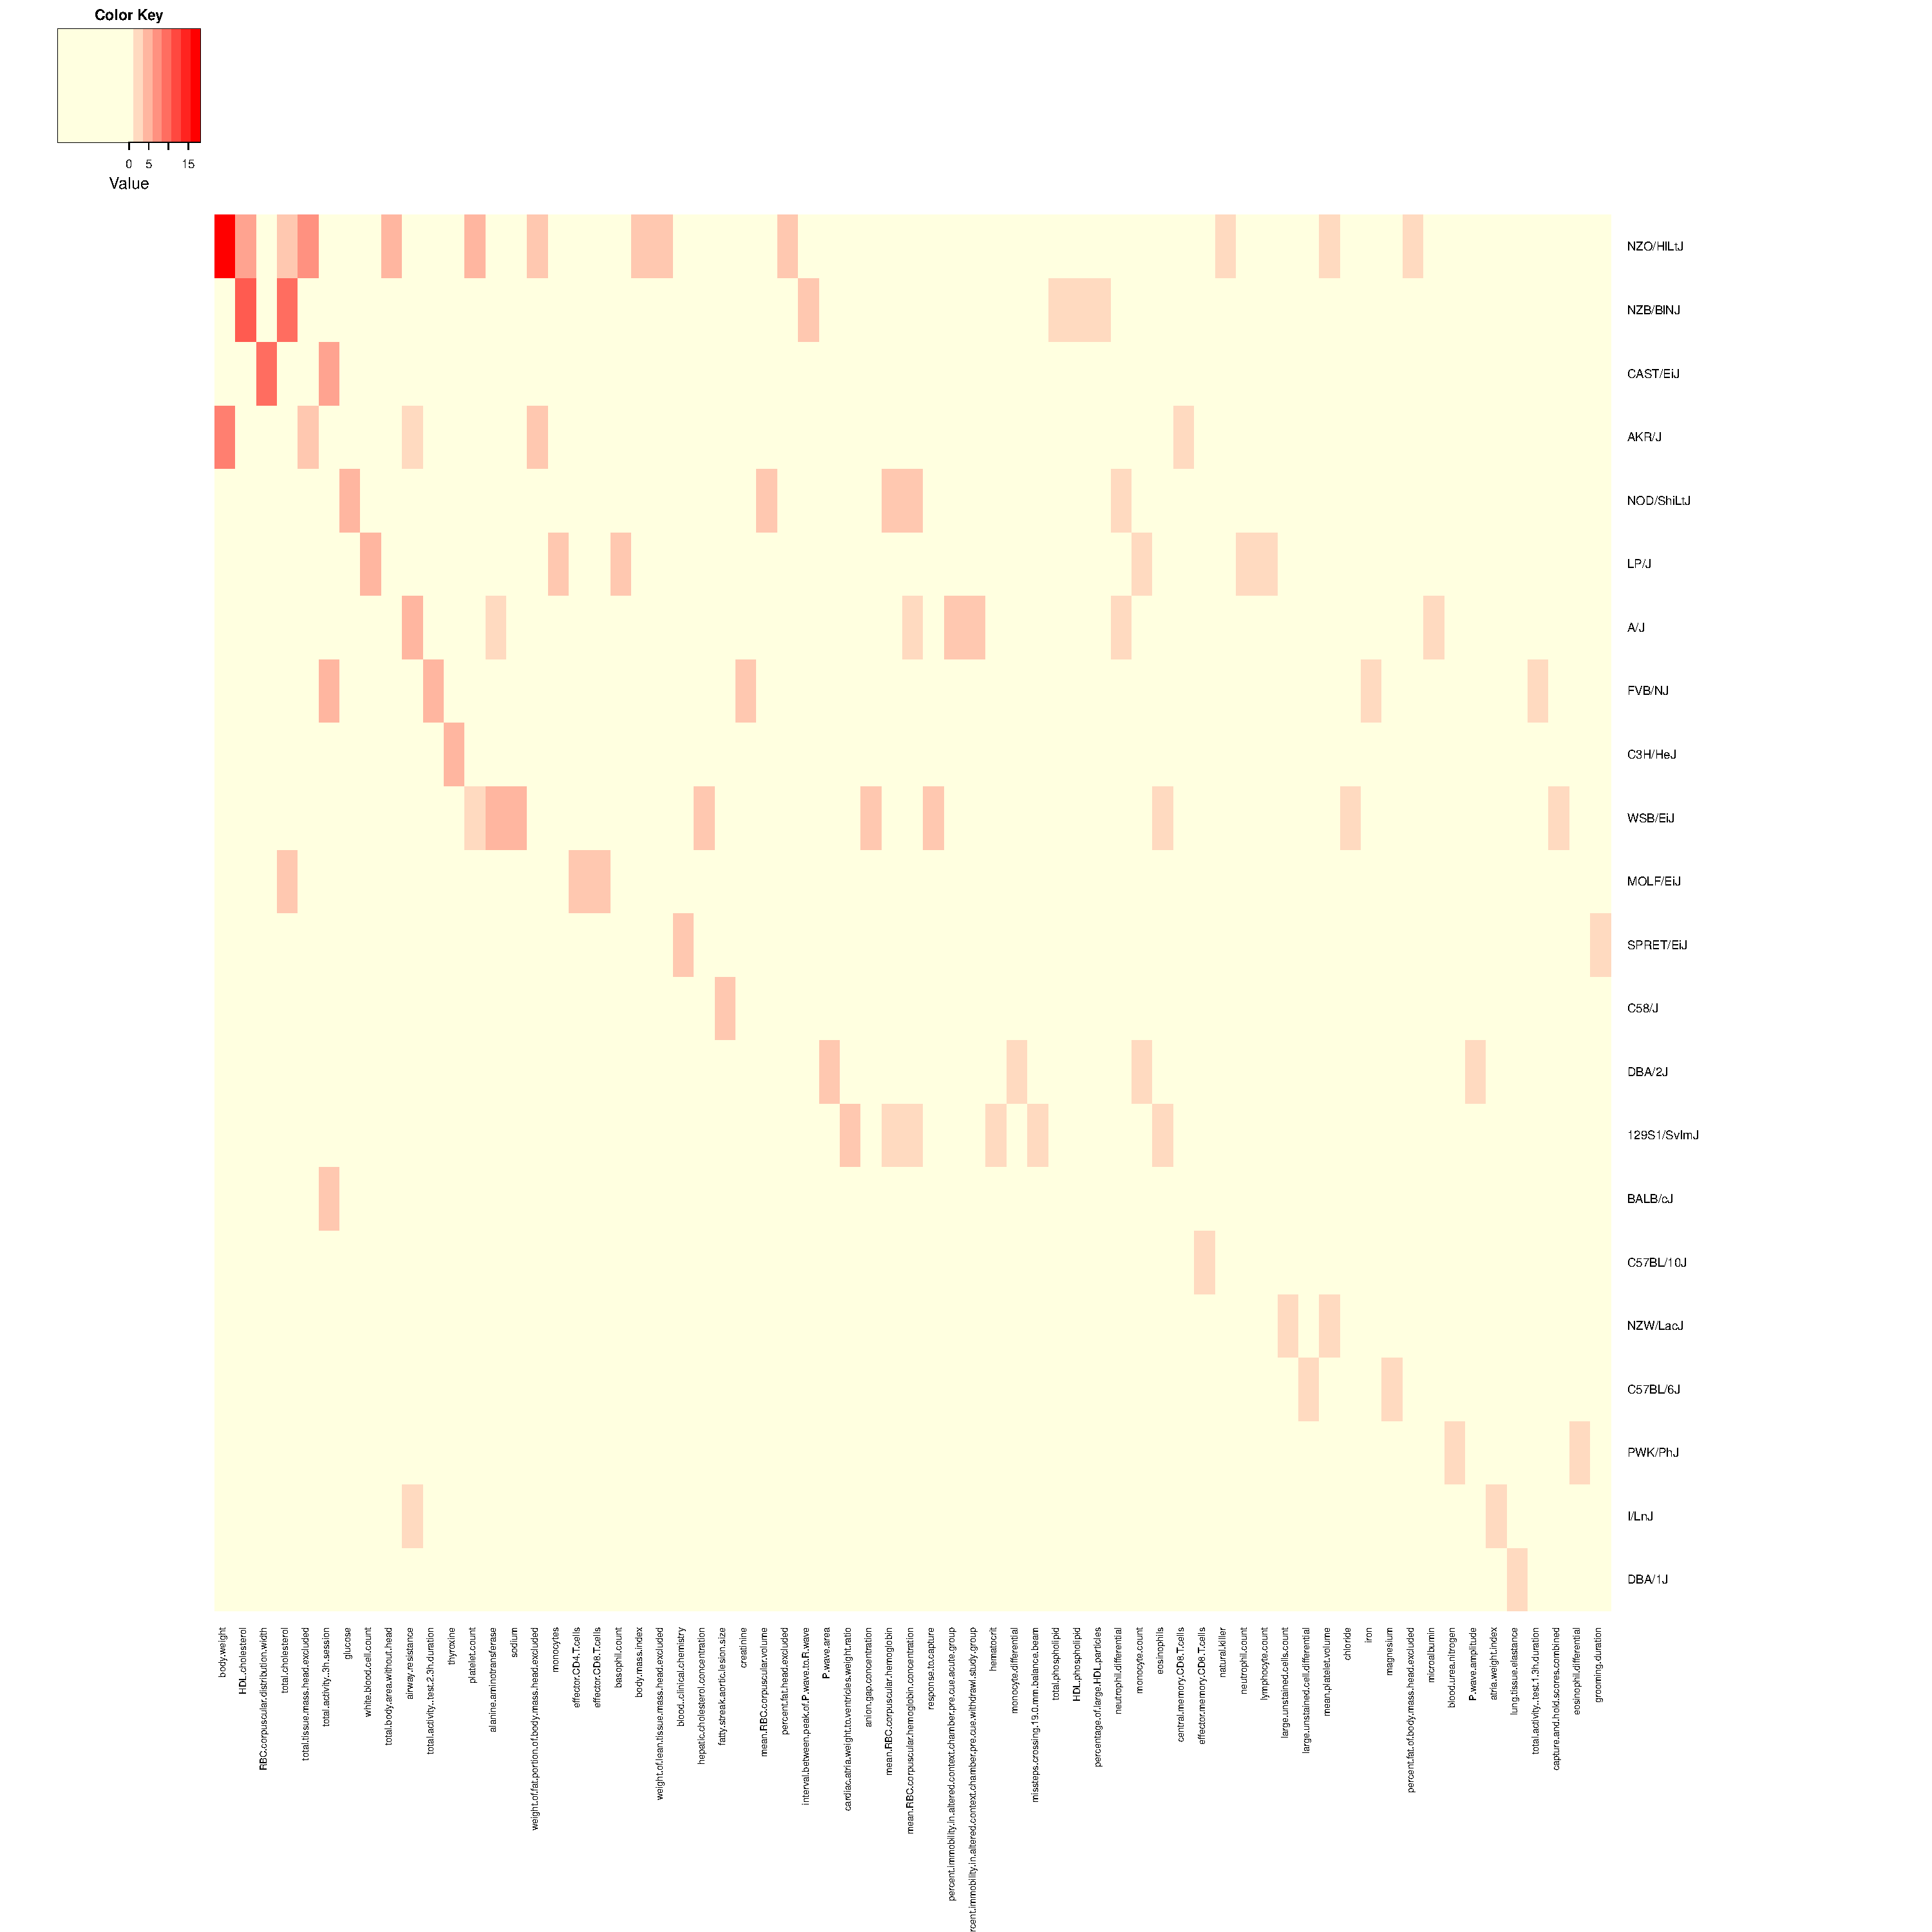
\includegraphics[width=\linewidth]{pics/mpi_phenotypes_strain_zscore2.pdf}
	\captionsetup{margin=12pt,format=plain,font=footnotesize,labelfont=bf}
 	\caption{\footnotesize{\textbf{MPD phenotype - strain associations, having Z-score $>$ 2}. 
	~~~~~~~\\
	Mouse Phenome Database phenotype occurrence frequency among the strains associated with the nuclear receptors, having Z-score $>$ 2}}
	\label{fig:mgi_pheotypes_strain_zscore2}
\end{figure}
~~~~~~~\\

\begin{figure}[H]
	\centering
	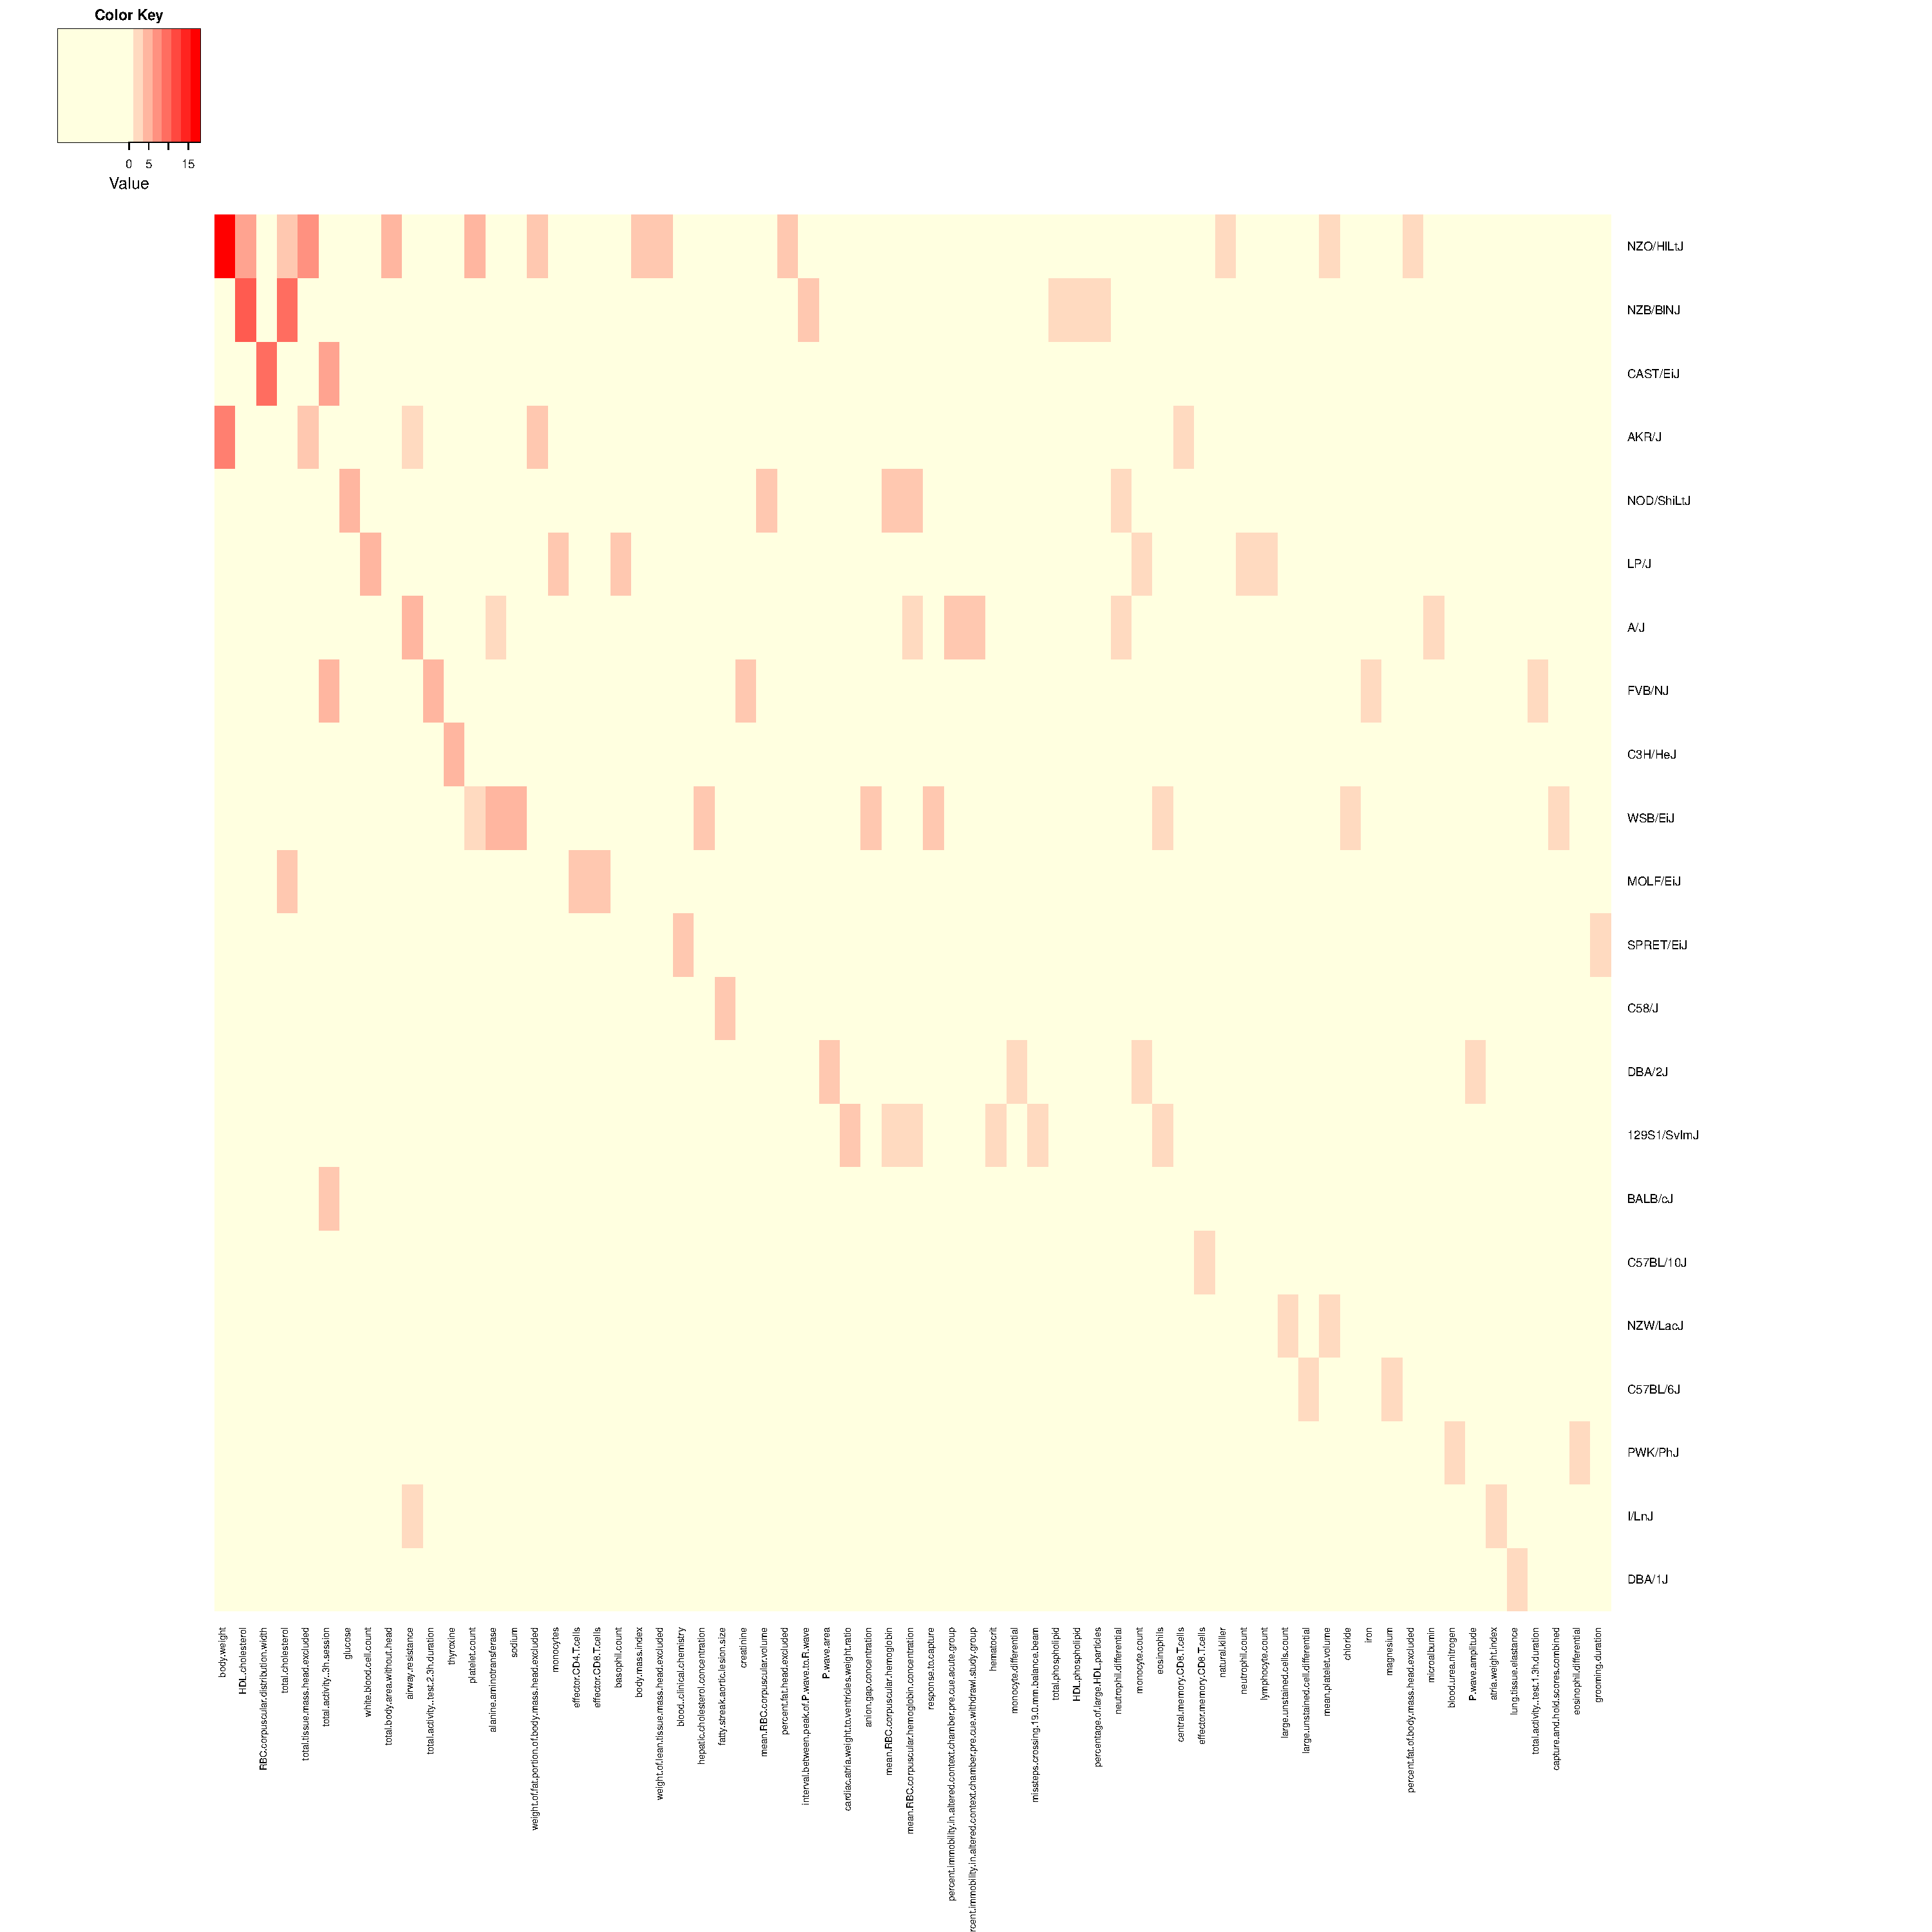
\includegraphics[width=\linewidth]{pics/mpi_phenotypes_strain_zscore2.pdf}
	\captionsetup{margin=12pt,format=plain,font=footnotesize,labelfont=bf}
 	\caption{\footnotesize{\textbf{MPD phenotype - strain associations, having Z-score $<$ -2}. 
	~~~~~~~\\
	Mouse Phenome Database phenotype occurrence frequency among the strains associated with the nuclear receptors, having Z-score $<$ -2}}
	\label{fig:mgi_pheotypes_strain_zscore2_neg}
\end{figure}

%------------------------------------------------
\section{Discussion and Outlook}

Blabla 

%------------------------------------------------
\section{Acknowledgments} % The \section*{} command stops section numbering

Our gratitude to Prof. Dr. H. W. Mewes for offering us the topic and the opportunity to work with the Helmholz Zentrum research centre in Munich. Many thanks to our supervisor, Dr. Desislava Boyanova for all the input and ideas, discussions, advices and foremost her useful and critical suggestions which motivated us a lot. Last but not least, we would like to thank our fellow colleagues for their support, as well as the entire \emph{Helmholz Zentrum} group. 
%----------------------------------------------------------------------------------------
%	REFERENCE LIST
%----------------------------------------------------------------------------------------
\phantomsection
\bibliographystyle{unsrt}
\bibliography{sample}

%----------------------------------------------------------------------------------------

\end{document}